\documentclass[color=usenames,dvipsnames]{beamer}

\mode<presentation> {

\usetheme{Madrid}
\usecolortheme{lily}
\useoutertheme{infolines}
}
\usepackage{booktabs} 
\usepackage{tikz}
\usepackage{subfigure}
% Thin fonts
\usepackage{cmbright}
\usepackage[T1]{fontenc}

\definecolor{dark_grey}{gray}{0.5}
\setbeamercolor{normal text}{fg=dark_grey,bg=white}
\setbeamertemplate{navigation symbols}{}

\setbeamercolor*{palette primary}{fg=gray!100,bg=gray!10}
\setbeamercolor*{palette quaternary}{fg=gray!100,bg=gray!10}
\setbeamercolor*{palette secondary}{fg=gray!100,bg=gray!20}
\setbeamercolor*{palette tertiary}{fg=gray!100,bg=gray!10}
\setbeamercolor*{navigation symbols}{fg=white,bg=white}
\usefonttheme{default}


\setbeamertemplate{blocks}[rounded][shadow=false]
\setbeamercolor{block title}{bg=gray!10}
\setbeamercolor{block body}{fg=gray,bg=gray!10}
%\setbeamercolor{frametitle}{fg=}

\setbeamertemplate{frametitle}[default][center]

\setbeamertemplate{itemize items}[default]
\setbeamertemplate{enumerate items}[default]


\newcommand{\F}{\mathbb{F}}
\setbeamertemplate{caption}[numbered]

\title[Software Plagiarism Check]{Parametrized String Matching Implementation for Software Plagiarism Check}
\author[]{Amit Tomar (MT2013008) \\Siddhesh Dosi  (MT2013150)\\ Srinivas R. Vaidya  (MT2013152) }

%\vskip .2 cm \fontsize{.3cm}{1em}\selectfont (Under the guidance of Prof. Jaya Sreevalsan Nayar)} 

\institute[IIIT-Bangalore]{International Institute of Information Technology, Bangalore}
\date{April 15, 2014}
\begin{document}

\begin{frame}
  \titlepage
\end{frame}

% Uncomment these lines for an automatically generated outline.
%\begin{frame}{Outline}
%  \tableofcontents
%\end{frame}

\section{Introduction}

\begin{frame}{Objective}

\begin{itemize}

  \setlength{\itemsep}{10pt}
  
\item This project aims at developing a Parametrized String Matching Implementation for Software Plagiarism Check, that given a collection of files which contain code in some programming language, will show a set of possible duplications of parts of the code among these. 
  
\item Comparing pieces of software will require discounting comments (optional and language dependent), extra/blank lines and spaces, variable renaming etc. 
  
\item The theory of parametrized string matching will be used to implementation this project. 

\item  System will have an easy-to-use UI for selecting files/folders and shall report the plagiarism related information (matches found) in the UI in a nice manner.

\end{itemize}
\end{frame}





\section{Functionality}

\begin{frame}{Functionality}

\begin{itemize}

\setlength{\itemsep}{30pt}
  
\item Plagiarism check among two given files. 
  
\item Pairwise plagiarism check among all the files in a given folder. 

\item Ignoring a code snippet for plagiarism check.

\end{itemize}
\end{frame}


\section{Technology}

\begin{frame}{Technology}

\begin{itemize}
  \setlength{\itemsep}{10pt}
  
  \item Exploring C++ / Python as option. 

  
\end{itemize}

\end{frame}

 


\section{Standard to be followed}

\begin{frame}{Coding standard to be followed}

\begin{figure}[h!]  
  \centering
  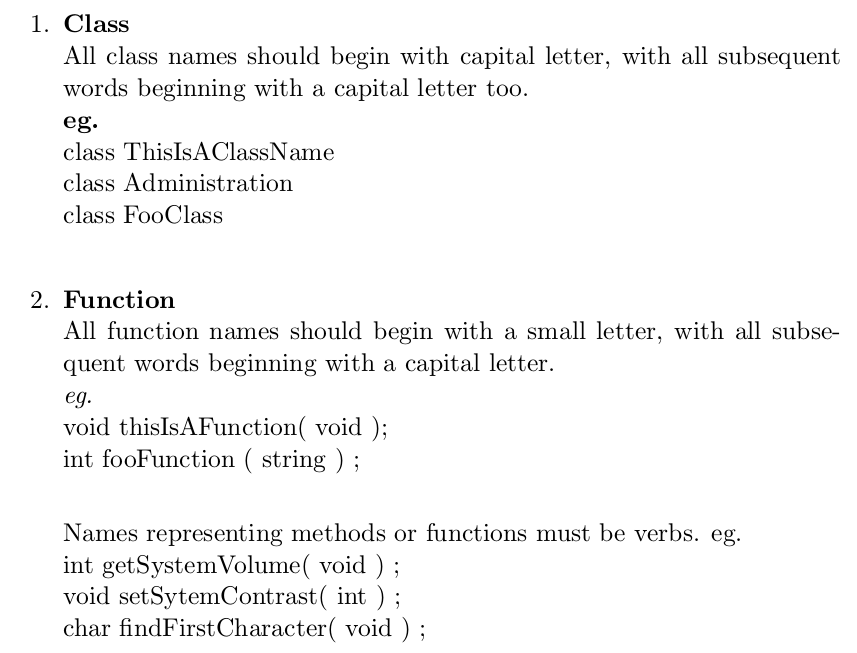
\includegraphics[width=.85\textwidth]{1.png}  
  \end{figure} 
\end{frame}

\section{Standard to be followed}

\begin{frame}{Coding standard to be followed}

\begin{figure}[h!]  
  \centering
  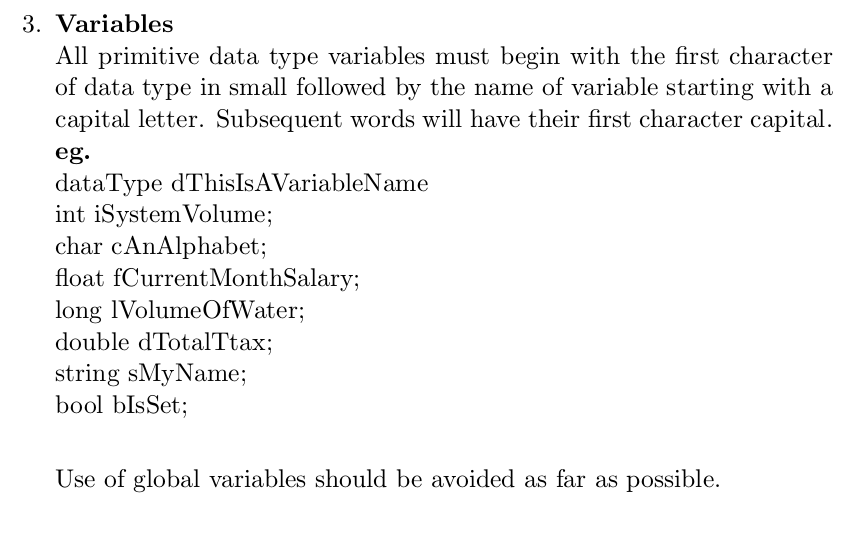
\includegraphics[width=.9\textwidth]{2.png}  
  \end{figure} 
\end{frame}

\section{Standard to be followed}

\begin{frame}{Coding standard to be followed}

\begin{figure}[h!]  
  \centering
  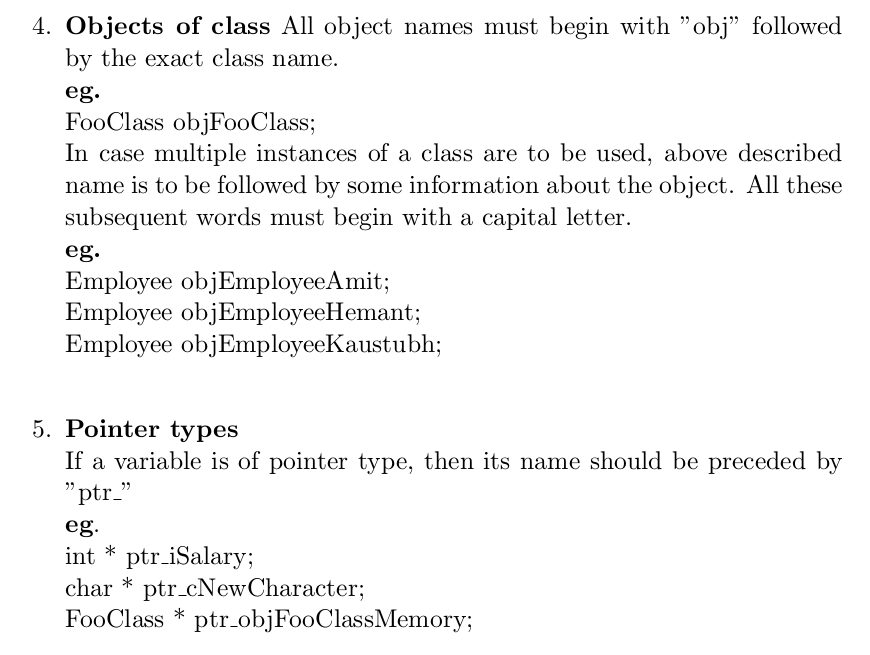
\includegraphics[width=.85\textwidth]{3.png}  
  \end{figure} 
\end{frame}

\section{Standard to be followed}

\begin{frame}{Coding standard to be followed}

\begin{figure}[h!]  
  \centering
  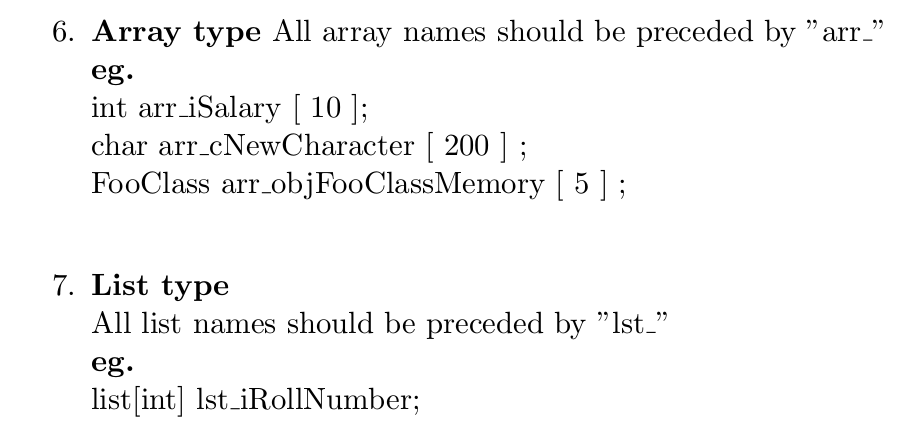
\includegraphics[width=.9\textwidth]{4.png}  
  \end{figure} 
\end{frame}


\section{Brief summary of work done}

\begin{frame}{Brief summary of work done}

\begin{itemize}
  \setlength{\itemsep}{25pt}

  \item \textbf{Requirement Specification} : Date of submission : 7 - Feb - 2014
(Already submitted to Prof. Srinivasraghvan)

\item \textbf{Literature Survey} : Expected date of completion : 20 - April - 2014
Expected time : 40 Hours
\end{itemize}

\end{frame}


\section{Plan for remaining work}

\begin{frame}{Plan for remaining work}

\begin{itemize}
  \setlength{\itemsep}{5pt}

  \item \textbf{Building suffix tree data structure} :
Expected date of completion : 15-May-2014,
Expected time : 30 Hours

\item \textbf{Identifying duplicate code using suffix tree}:
Expected date of completion : 1-June-2014,
Expected time : 25 Hours

\item \textbf{Implementation of UI}:
Expected date of completion : 10-June-2014, 
Expected time : 10 Hours

\item \textbf{Parameterized implementation for software plagiarism
check}:
Expected date of completion : 1-July-2014,
Expected time : 40 Hours

\item \textbf{Integration of UI with parameterized string matching
code}:
Expected date of completion : 15-July-2014,
Expected time : 20 Hours

\item \textbf{Testing}:
Expected date of completion : 31-July-2014,
Expected time : 20 Hours

\end{itemize}

\end{frame}


\section{Tools used}

\begin{frame}{Tools used}

\begin{figure}[h!]  
  \centering
  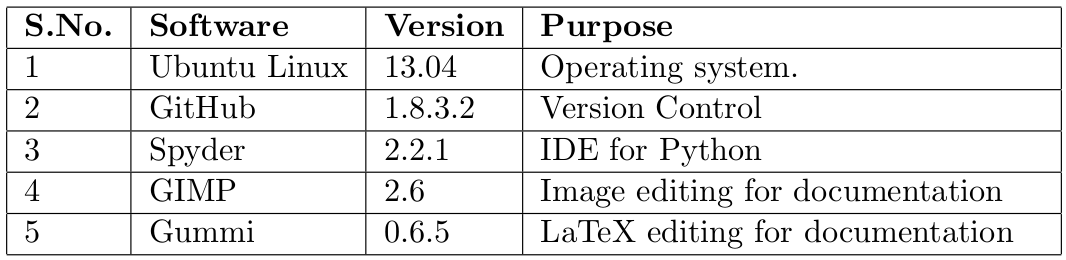
\includegraphics[width=1\textwidth]{5.png}  
  \end{figure} 
\end{frame}


\section{References}

\begin{frame}{References}

\begin{itemize}

  \setlength{\itemsep}{20pt}

\fontsize{.25cm}{1em}\selectfont

\item  [1]	Peter Vamplew, Julian Dermoudy, \emph{An Anti-Plagiarism Editor for Software Development Courses}, Proceeding ACE-05 Proceedings of the 7th
Australasian conference on Computing education - Volume 42 Pages 83-
90 , 2005.

\end{itemize}

\end{frame}

\end{document} 